\chapter{Ejercicio 2}

\section{Actividad 1}

\subsection{A}

\textbf{A)} Expresar la Ecuación Diferencial (ED) que describe el circuito, y con ello, definir un
Sistema en tiempo continuo con entrada x(t) = v(t) y salida y(t) = i(t) , con condiciones
Iniciales genérica (CI).

\begin{figure}[H]
  \centering
  \begin{circuitikz}[american voltages]
    \node at (-3,1) {ENTRADA};
    \node at (-3,0) {$x(t) = v(t)$};
    
    \draw (-1,-1) rectangle (3.5,2.5);

    \draw (-0.5,1.5) to[R=$R$] (2,1.5)
          to[C=$C$] (2,-0.5) -- (-0.5,-0.5);
    
    \draw[->] (-4, 0.5) -- (-1,0.5);

    \node at (6,1) {SALIDA};
    \node at (6,0) {$y(t) = i(t)$};
    
    \draw[->] (3.5,0.5) -- (6,0.5);
  \end{circuitikz}
\end{figure}

Para plantear la EDO es necesario plantear ley de kirchoff

$$v(t) = R \cdot i(t) + \dfrac{1}{C} \cdot \int i(t) dt$$

Ahora derivamos para conseguir la expresion buscada

$$\dfrac{d v(t)}{dt} = R \dfrac{d i(t)}{dt} + \dfrac{1}{C} \cdot i(t)$$

Dividimos todo por $R$ para normalizar la ecuacion

$$\dfrac{d i(t)}{dt} + \dfrac{1}{RC} \cdot i(t) = \dfrac{1}{R} \cdot \dfrac{d v(t)}{dt}$$

$$y'(t) + \dfrac{1}{RC} \cdot y(t) = \dfrac{1}{R} \cdot x'(t)$$

Para el circuito de segundo orden:

\begin{figure}[H]
  \centering
  \begin{circuitikz}[american voltages]
    \node at (-3,1) {ENTRADA};
    \node at (-3,0) {$x(t) = v(t)$};
    
    \draw (-1,-1) rectangle (3.5,2.5);

    \draw (-0.5,1.5) to[R=$R$] (1.25,1.5) to[L=$L$] (2.3,1.5)
          to[C=$C$] (2.3,-0.5) -- (-0.5,-0.5);
    
    \draw[->] (-4, 0.5) -- (-1,0.5);

    \node at (6,1) {SALIDA};
    \node at (6,0) {$y(t) = i(t)$};
    
    \draw[->] (4,0.5) -- (6,0.5);
  \end{circuitikz}
\end{figure}

Siguiendo con el mismo procedimiento

$$v(t) = R \cdot i(t) + L \cdot \dfrac{d i(t)}{dt} + \dfrac{1}{C} \cdot \int i(t) dt$$

$$\dfrac{d v(t)}{dt} = R \cdot \dfrac{d i(t)}{dt} + L \cdot \dfrac{d^2 i(t)}{dt^2} + \dfrac{1}{C} \cdot i(t)$$

$$\dfrac{d^2 i(t)}{dt^2} +  \dfrac{R}{L} \cdot \dfrac{d i(t)}{dt} + \dfrac{1}{LC} \cdot i(t) = \dfrac{1}{L} \cdot \dfrac{d v(t)}{dt} $$

$$y''(t) + \dfrac{R}{L} \cdot y'(t) + \dfrac{1}{LC} \cdot y(t) = \dfrac{1}{L} \cdot x'$$

\subsection{B}

\textbf{B)}Usar la transformada de Laplace para sintetizar el sistema en la expresión

Primero sintetizamos la ecuacion correspondiente al circuito de primer orden

$$\mathscr{L}[y'(t)] = sY(s) - y(0)$$

$$\mathscr{L}[y(t)] = Y(s)$$

$$\mathscr{L}[x'(t)] = sX(s) - x(0)$$

Quedando la ecuacion

$$sY(s) - y(0) + \dfrac{1}{RC} \cdot Y(s) = \dfrac{1}{R} \cdot (sX(s) - x(0))$$

$$Y(s) (s + \dfrac{1}{rc}) = \dfrac{1}{R} \cdot sX(s) - \dfrac{1}{R} x(0) + y(0)$$

$$Y(s) = X(s)  \dfrac{\dfrac{s}{R}}{s + \dfrac {1}{RC}} + \dfrac{1}{(s + \dfrac{1}{RC})} [y(0) - x(0) \dfrac{1}{R}]$$

Ya nos queda sintetizado a la expresion

$$Y(s) = X(s) \cdot H(s) + F(s,CI)$$

Ahora para el circuito de segundo orden, primero debemos definir la transformada para la segunda derivada

$$\mathscr{L}[y''(t)] = s^2Y(s) - sy(0) - y'(0)$$

Quedando la ecuacion sintetizada

$$ s^2Y(s) - s y(0) - y'(0) + \dfrac{R}{L} (sY(s) - y(0)) + \dfrac{1}{LC} \cdot Y(s) = \dfrac{1}{L} \cdot (sX(s) - x(0))$$

$$ Y(s) (s^2 + \dfrac{R}{L} s + \dfrac{1}{LC}) = X(s) \dfrac{s}{L} - x(0) \dfrac{1}{L} + s y(0) + y'(0) + \dfrac{R}{L} y(0)$$

$$ Y(s) = X(s) \dfrac{\dfrac{s}{L}}{s^2 + \dfrac{R}{L} s + \dfrac{1}{LC}} + \dfrac{1}{s^2 + \dfrac{R}{L} s + \dfrac{1}{LC}} [s y(0) + y'(0) + \dfrac{R}{L} y(0) - x(0) \dfrac{1}{L}]$$

\subsection{C}

\textbf{C)} Escribir un diagrama de Bloques en la variable compleja S que determine al Sistema.

El diagrama de bloques que describe a la ecuacion de primer orden es:

\begin{figure}[H]
  \centering
  \begin{circuitikz}
    \node at (-2.5,1) {$X(s)$};
    \draw[->] (-3,0.5) -- (0,0.5);

    \draw (0,1) rectangle (1,0);

    \node at (0.5,0.5) {$H(s)$};
  
    \draw (1,0.5) -- (3,0.5);
    \draw[->] (3,0.5) -- (3,-0.5);

    \node at (-2.5,-2) {$F(s,CI)$};
    \draw[->] (-3,-2.5) -- (0,-2.5);

    \draw (0,-1.87) rectangle (1.25,-3.12);
    
    \draw (1.25,-2.5) -- (3,-2.5);
    \draw[->] (3,-2.5) -- (3,-1);

    \node[scale=0.7] at (0.625,-2.475) {$\dfrac{1}{s+\dfrac{1}{RC}}$};

    \draw (3,-0.75) circle (0.25cm);

    \node at (3,-0.75) {+};

    \draw[->] (3.25,-0.75) -- (4.25,-0.75);
    \node at (4,-0.25) {$Y(s)$};
  \end{circuitikz}
\end{figure}

Por otro lado el que describe a la ecuacion de segundo orden

\begin{figure}[H]
  \centering
  \begin{circuitikz}
    \node at (-2.5,1) {$X(s)$};
    \draw[->] (-3,0.5) -- (0,0.5);

    \draw (0,1) rectangle (1,0);

    \node at (0.5,0.5) {$H(s)$};
  
    \draw (1,0.5) -- (3,0.5);
    \draw[->] (3,0.5) -- (3,-0.5);

    \node at (-2.5,-2) {$F(s,CI)$};
    \draw[->] (-3,-2.5) -- (0,-2.5);

    \draw (0,-1.87) rectangle (1.25,-3.12);
    
    \draw (1.25,-2.5) -- (3,-2.5);
    \draw[->] (3,-2.5) -- (3,-1);

    \node[scale=0.45] at (0.625,-2.475) {$\dfrac{\dfrac{s}{L}}{s^2+\dfrac{R}{L}s+\dfrac{1}{LC}}$};

    \draw (3,-0.75) circle (0.25cm);

    \node at (3,-0.75) {+};

    \draw[->] (3.25,-0.75) -- (4.25,-0.75);
    \node at (4,-0.25) {$Y(s)$};
  \end{circuitikz}
\end{figure}

\subsection{D}

\textbf{D)} Graficar en el plano $S$ polos y ceros de $H(s)$.

Para el caso de primer orden

$$H(s) = \dfrac{\dfrac{s}{R}}{s + \dfrac{1}{RC}}$$

Donde el unico polo se encuentra en $s=-\dfrac{1}{RC}$ y el cero en $s=0$.

$R = 3$, $C = \dfrac{1}{2}$, $L = 1$.

El polo con estos datos seria $s=-\dfrac{2}{3}$

\begin{figure}[H]
  \centering
  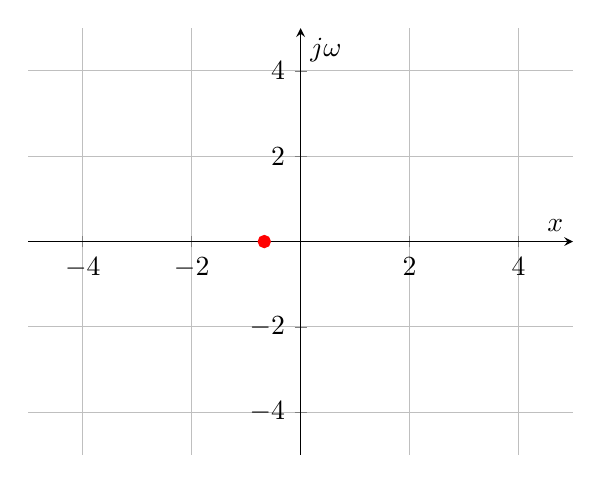
\begin{tikzpicture}
    \begin{axis}[
        axis lines=middle,
        xlabel={$x$},
        ylabel={$j\omega$},  
        grid=both,
        width=8.5cm,
        height=7cm,
        ymin=-5, ymax=5,
        xmin=-5, xmax=5,
      ]
      \addplot[red, thick, mark=*] coordinates {(-2/3,0)};
    \end{axis}
  \end{tikzpicture}
\end{figure}

Para la ecuacion de segundo orden 

$$H(s) = \dfrac{\dfrac{s}{L}}{s^2 + \dfrac{R}{L} s + \dfrac{1}{LC}}$$

Y los polos se encontrarian en $s_n=\dfrac{-\dfrac{R}{L} \pm \sqrt{\dfrac{R}{L}^2-\dfrac{4}{LC}}}{2}$

Donde reemplazando con los valores previamente dados, los polos quedarian en $(-1,0)$ y $(-2,0)$.

\begin{figure}[H]
  \centering
  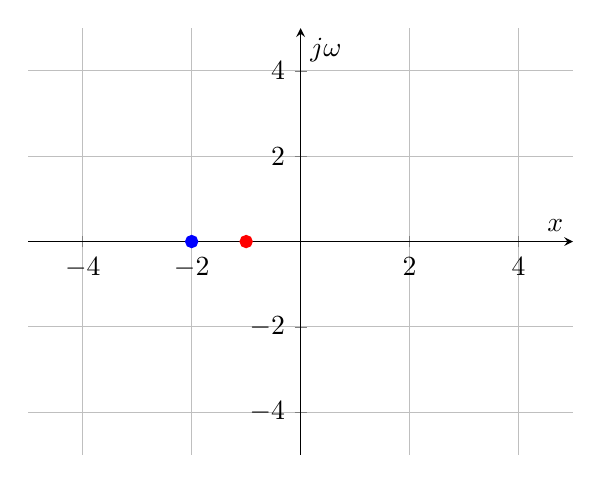
\begin{tikzpicture}
    \begin{axis}[
        axis lines=middle,
        xlabel={$x$},
        ylabel={$j\omega$},  
        grid=both,
        width=8.5cm,
        height=7cm,
        ymin=-5, ymax=5,
        xmin=-5, xmax=5,
      ]
      \addplot[red, thick, mark=*] coordinates {(-1,0)};
      \addplot[blue, thick, mark=*] coordinates{(-2,0)};
    \end{axis}
  \end{tikzpicture}
\end{figure}

\subsection{E}

\textbf{E)} Obtener la respuesta al impulso, $h(t)$, suponiendo que las CI = 0.

Continuaremos resolviendo primero la ecuacion de primer orden

$$\mathscr{L} [\delta (t)] = 1$$

$$\mathscr{L}^{-1} [H(s) \cdot 1] = \mathscr{L} [H(s)]$$

$$H(s) = \dfrac{1}{R} \dfrac{s}{s + \dfrac{1}{RC}}$$

$$\dfrac{1}{RC} = a$$

$$H(s) = \dfrac{1}{R} \dfrac{s + a - a}{s + a}$$

$$H(s) = \dfrac{1}{R} (\dfrac{s + a}{s + a} - \dfrac{a}{s + a})$$

$$H(s) = \dfrac{1}{R} (1 - \dfrac{a}{s + a})$$

$$h(t) = \mathscr{L}^{-1} [\dfrac{1}{R} (1 - \dfrac{a}{s + a})] = \dfrac{1}{R} \mathscr{L}^{-1} [1 - \dfrac{a}{s + a}] = \dfrac{1}{R} (\mathscr{L}^{-1} [1] - \mathscr{L}^{-1} [\dfrac{a}{s + a}])$$

$$\mathscr{L}^{-1} [1] = \delta (t) $$

$$\mathscr{L}^{-1} [\dfrac{a}{s + a}] = a e^{-at} u(t)$$

$$h(t) = \dfrac {1}{R} (\delta (t) - a e^{at} u(t))$$

$$h(t) = \dfrac {1}{R} (\delta (t) - \dfrac{1}{RC} e^{\dfrac{1}{RC} t} u(t))$$

$$h(t) = \dfrac{\delta (t)}{3} - \dfrac{2}{9} e^{\frac{2}{3}} u(t)$$

Para la ecuacion de segundo orden

$$H(s) = \dfrac{\dfrac{s}{L}}{s^2 + \dfrac{R}{L} s + \dfrac{1}{LC}}$$

$$\dfrac{R}{L} = a; \dfrac{1}{LC} = b$$

$$H(s) = \dfrac{1}{L} \dfrac{s}{s^2 + a s + b}$$

$$H(s) = \dfrac{1}{L} \dfrac{s}{(s + 1) (s + 2)}$$

$$H(s) = \dfrac{1}{L} \frac{-1}{s + 1} + \frac{2}{s + 2} $$

$$h(t) = \mathscr{L}^{-1} [H(s)] = \mathscr{L}^{-1} [\frac{1}{L} \frac{-1}{s + 1} + \frac{2}{s + 2}]$$

$$h(t) = \frac{1}{L} \mathscr{L}^{-1} [\frac{-1}{s + 1} + \frac{2}{s + 2}]$$

$$h(t) = \frac{1}{L} (-\mathscr{L}^{-1} (\frac{1}{s + 1}) + \mathscr{L}^{-1} (\frac{2}{s + 2}))$$

$$h(t) = \frac{1}{L} (-e^{-t} u(t) + 2 e^{-2t} u(t))$$

$$h(t) = \frac{1}{L} u(t) (-e^{-t} + 2 e^{-2t})$$

\subsection{F}

\textbf{F)} Obtener la respuesta al escalón unitario $v(t)$, suponiendo CI = 0 y verificar la identidad $\frac{d}{dt} v(t) = h(t), \forall t$

Para la ecuacion de primer orden

$$v(t) = \mathscr{L}^{-1} (H(s) \cdot \mathscr{L} (u(t)))$$

$$v(t) = \mathscr{L}^{-1} (\dfrac{\dfrac{s}{R}}{s + \dfrac{1}{RC}} \cdot \dfrac{1}{s})$$

$$v(t) = \dfrac{1}{R} \mathscr{L}^{-1} (\dfrac{1}{s + \dfrac{1}{RC}})$$

$$\dfrac{1}{RC} = a $$

$$v(t) = \dfrac{1}{R} \mathscr{L}^{-1} (\dfrac{1}{s + a}) $$

$$v(t) = \dfrac{1}{R} e^{-at} u(t) $$

$$v(t) = \dfrac{1}{3} e^{-\dfrac{2}{3}t} u(t)$$

En el caso de la ecuacion de segundo orden

$$v(t) = \mathscr{L}^{-1} (\dfrac{\dfrac{s}{L}}{s (s + 1) (s + 2)})$$

$$v(t) = \dfrac{1}{L} \mathscr{L}^{-1} (\dfrac{1}{(s + 1)(s + 2)})$$

Por fracciones simples

$$v(t) = \dfrac{1}{L} \mathscr{L}^{-1} (\dfrac{A}{s + 1} \dfrac{B}{s + 2})$$

$$v(t) = \dfrac{1}{L} \mathscr{L}^{-1} (\dfrac{1}{s + 1} - \dfrac{1}{s + 2})$$

$$v(t) = \dfrac{1}{L} \mathscr{L}^{-1} (\dfrac{1}{s + 1}) - \mathscr{L}^{-1} (\dfrac{1}{s + 2})$$

$$v(t) = \dfrac{1}{L} (e^{-t} - e^{-2t}) u(t) $$

$$L=1$$

$$v(t) = (e^{-t} - e ^{-2t}) u(t)$$

Ahora para ambos casos vamos a verificar que $\dfrac{dv(t)}{dt} = h(t)$

En ambos casos vamos a usar que $\dfrac{d}{dt} [f(t)u(t)] = f(0)\delta (t) + f'(t) u(t)$, siendo para el la ecuacion de primer orden

$$v(0) = \dfrac{1}{3} $$

$$v'(t) = \dfrac{-2}{9} e^{-\dfrac{2}{3}}$$

Quedando

$$\dfrac{dv(t)}{dt} = \dfrac{\delta(t)}{3} - \dfrac{2}{9} e^{-\dfrac{2}{3}} u(t) $$

Por lo cual se verifica para la primera ecuacion, por otro lado para la segunda ecuacion

$$v(0) = e^{-0} - e^{0} = 1 - 1 = 0$$

$$v'(t) = e^{-t} + 2e^{-2t} $$

Lo cual aplicando lo explicado anteriormente

$$\dfrac{dv(t)}{dt} = 0 \delta(t) + e^{-t} + 2e^{-2t} u(t) $$

$$\dfrac{dv(t)}{dt} = e^{-t} + 2e^{-2t} u(t) = h(t)$$

\subsection{G}

\textbf{G)} Obtener la respuesta a la rampa.

Primero transformamos la integral del escalon

$$\mathscr{L} (\int_{-\infty}^{t} u(\tau) d\tau)$$

$$\mathscr{L} (\int_{-\infty}^{0} 0 d\tau + \int_{0}{t} 1 d\tau)$$

$$\mathscr{L} (t)$$

$$\mathscr{L} (t) = \dfrac{1}{s^2}$$

Entonces para calcular la respuesta a la rampa con la ecuacion de primer orden

$$y(t) = \mathscr{L}^{-1} (H(s)\dfrac{1}{s^2})$$

$$y(t) = \mathscr{L}^{-1} (\dfrac{\dfrac{s}{R}}{s + \dfrac{1}{RC}} \cdot \dfrac{1}{s^2})$$

$$y(t) = \dfrac{1}{R} \mathscr{L}^{-1} (\dfrac{1}{s(s + \dfrac{1}{RC})})$$

$$\dfrac{1}{RC} = \dfrac{2}{3} = a$$

$$y(t) = \dfrac{1}{R} \mathscr{L}^{-1} (\dfrac{A}{s} + \dfrac{B}{s + a}) $$

$$A=\dfrac{1}{a}; B=-\dfrac{1}{a} $$

$$y(t) = \dfrac{1}{R} \dfrac{1}{a} \mathscr{L}^{-1}(\dfrac{1}{s} - \dfrac{1}{s+a}) $$

$$y(t) = \dfrac{1}{R} \dfrac{1}{a} (\mathscr{L}^{-1}\dfrac{1}{s} - \mathscr{L}^{-1}\dfrac{1}{s+a})$$

$$y(t) = \dfrac{1}{R} \dfrac{1}{a} (u(t) - e^{-at}u(t))$$

$$y(t) = \dfrac{1}{aR} u(t) (1 - e^{-at})$$

$$y(t) = C u(t) (1 - e^{-\dfrac{1}{RC}t}) $$

$$y(t) = \dfrac{1}{2} u(t) (1 - e^{-\dfrac{2}{3}t}) $$

Para el caso de la ecuacion de segundo orden, recordamos que

$$H(s) = \dfrac{\dfrac{s}{L}}{s^2 + \dfrac{R}{L} s + \dfrac{1}{LC}}$$

$$y(t) = \mathscr{L}^{-1} (\dfrac{\dfrac{s}{L}}{s^2 + \dfrac{R}{L} s + \dfrac{1}{LC}} \cdot \dfrac{1}{s^2})$$

$$y(t) = \dfrac{1}{L} \mathscr{L}^{-1} (\dfrac{1}{s(s^2 + \dfrac{R}{L} s + \dfrac{1}{LC})}) $$

$$y(t) = \dfrac{1}{L} \mathscr{L}^{-1} (\dfrac{1}{s(s+1)(s+2)}) $$

$$y(t) = \dfrac{1}{L} \mathscr{L}^{-1} (\dfrac{A}{s} + \dfrac{B}{s+1} + \dfrac{C}{s+2})$$

$$y(t) = \dfrac{1}{L} \mathscr{L}^{-1} (\dfrac{\dfrac{1}{2}}{s} - \dfrac{1}{s+1} + \dfrac{\dfrac{1}{2}}{s+2}) $$

$$y(t) = \dfrac{1}{L} [\dfrac{1}{2} \mathscr{L}^{-1} (\dfrac{1}{s}) - \mathscr{L}^{-1} (\dfrac{1}{s+1}) + \dfrac{1}{2} \mathscr{L}^{-1} (\dfrac{1}{s+2})] $$

$$y(t) = \dfrac{1}{L} [\dfrac{1}{2} u(t) - e^{-t} u(t) + \dfrac{1}{2} e^{-2t} u(t)] $$

$$y(t) = \dfrac{1}{L} u(t) [\dfrac{1}{2} - e^{-t} + \dfrac{e^{-2t}}{2}]$$

$L = 1$

$$y(t) = u(t) [\dfrac{1}{2} - e^{-t} + \dfrac{e^{-2t}}{2}] $$

Vamos a completar este ejercicio realizando al verificacion de los calculos mediante la siguiente igualdad $y(t) = \int_{-\infty}^{t} v(\tau) d\tau$.

Manteniendo el orden de realizacion de ejercicios, comenzamos con la ecuacion de primer orden

$$v(t) = \dfrac{1}{3} e^{-\dfrac{2}{3}t} u(t)$$

$$\int_{-infty}^{t} v(t) = \dfrac{1}{3} \int_{0}^{t} e^{-\dfrac{2}{3}\tau} d\tau = y(t) $$

$a = \dfrac{-2}{3}$

$$y(t) = \dfrac{1}{3} [\dfrac{1}{a} e^{at} \bigg\rvert_{0}^{t}] $$

$$y(t) = \dfrac{1}{3} \dfrac{1}{a} (e^{at} - 1) $$

$$y(t) = -\dfrac{1}{2} e^{-\dfrac{2}{3}t} - \dfrac{1}{2} $$

$$y(t) = \dfrac{1}{2} (1 - e^{-\dfrac{2}{3}t}) $$ 

Verificando correctamente para la primera ecuacion, ahora correspondemos con la de segundo orden

$$v(t) = (e^{-t} - e^{-2t}) u(t) $$

$$\int_{-\infty}^{t} v(t) = y(t) $$

$$\int_{-\infty}^{t} v(t) = \int_{0}^{t} (e^{-\tau} - e^{-2\tau}) d\tau $$

$$\int_{-\infty}^{t} v(t) = \int_{0}^{t} e^-{-\tau} d\tau - \int_{0}^{t} e^{-2\tau} d\tau $$ 

$$\int_{-\infty}^{t} v(t) = -e^{-\tau}\bigg\rvert_{0}^{t} - (-\dfrac{1}{2} e^{-2\tau} \bigg\rvert_{0}^{t}) $$

$$\int_{-\infty}^{t} v(t) = -(e^{-t} - 1) - (-\dfrac{1}{2} e^{-2t} + \dfrac{1}{2}) $$

$$\int_{-\infty}^{t} v(t) = 1 - e^{-t} + \dfrac{1}{2} e^{-2t} - \dfrac{1}{2}$$

$$\int_{-\infty}^{t} v(t) = \dfrac{1}{2} - e^{-t} + \dfrac{1}{2} e^{-2t}$$

Su forma causal

$$\int_{-\infty}^{t} v(t) = u(t) [\dfrac{1}{2} - e^{-2t} + \dfrac{1}{2} e^{-2t}]$$

Por lo cual se verifica todo lo calculado anteriormente
